\section{System Design}
\label{sec:design}

\subsection{Overview}
In designing Vivian, we want the system to achieve the following properties:

\begin{itemize}
    \item \textbf{Decentralized Naming and Look-up.} End-users can register for and bind values to human-meaningful names and look up the values of names without relying on the trust of central authorities.
    \item \textbf{Decentralized and Secure Storage.} End-users can store their data in a decentralized manner. Besides, users can control the access rights of their data.
    \item  \textbf{IoT Device Supported.} The whole process like registering a name, looking up a name, and file handling should not be energy-hungry or hardware resource hungry.
          They can be accomplished by devices with limited hardware resources such as Raspberry Pi.
\end{itemize}

The overall architecture of Vivian can be divided into three layers: \textbf{Tangle DL layer, Peer Network layer, and Storage layer}.
Tangle distributed ledger is used as storage intermediate of critical data binding and for consensus of the order of the system operations.
Nodes in the peer network layer are equally privileged, equipotent peers which perform the live listening to transactions on Tangle, parsing the operations, storing naming key-value pairs, and routing for users to find the information of the names.
Storage layer is an alternative layer for users to store the name pointing data. Overview of the architecture is shown in Fig~\ref{fig:vivian_architecture}.

\begin{figure}[h]
    \centering
    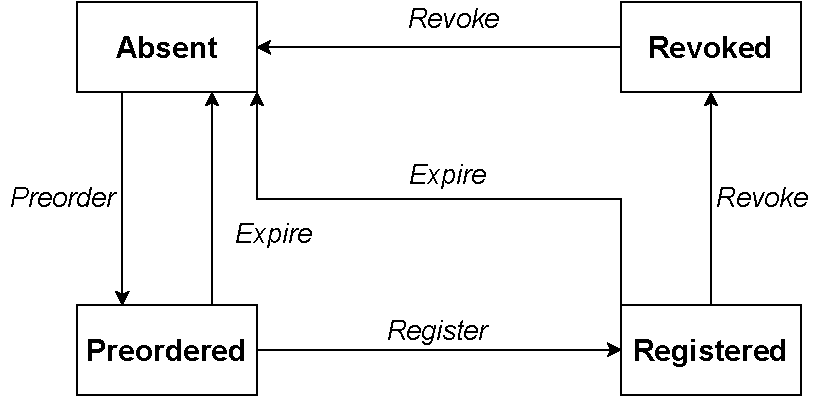
\includegraphics[width=0.4\textwidth,trim={0 0 0 0},clip]{figs/name_state_transition.pdf}
    \caption{Name state transitions}
    \label{fig:name_state_transition}
\end{figure}

\subsection{Naming System}
The design of the naming system is inspired by the implementation of Namecoin \cite{kalodner2015empirical} and BNS of Blockstack \cite{ali2017blockstack, ali2016blockstack}.
Names are owned by the cryptographic public addresses and the corresponding seed which generates the address of IOTA. In IOTA, addresses are generated by the user's private seed with Kerl Hash Function \cite{Baek2019IOTAAC}. As shown in Fig~\ref{fig:name_state_transition}, operations in the naming system perform the state transitions of names.
Each name has four states: \textbf{absent, preordered, registered, and revoked}. And \textbf{preorder, register, revoke, and expire} operations transit the state of the name into one another. In addition, as a registered name, \textbf{renew, update, and transfer} operations can be performed for changing its binding value.

To claim a name, a user needs to first preorder the target name and then register it. Preorder operation is for users to indicate interest in the name. The operation sends a transaction with the message containing the hash commitment of desired name rather than plain text. The reason for sending hash commitment is to prevent front-running \cite{kalodner2015empirical}, e.g., if a name is revealed to the public, an attacker can race the user for claiming it \cite{ali2016blockstack}.
The preorder operation also acts as a signal for the nodes in the peer network to start the preprocessing of a name registration.
After preorder, the user can send the register operation for providing the name he/she wants to claim, the transaction hash of the previous preorder transition, the keys for decrypting the hash commitment, and the value for name binding.
The first user who finishes both preorder and register operation successfully will grant ownership of the name.
And any preorder operations performed by the other users will be invalid. In Namecoin's implementation, \texttt{NAME\_NEW} and \texttt{NAME\_FIRSTUPDATE} operations are equivalent to the preorder and register operations in Vivian.
For the effectiveness of \texttt{NAME\_NEW} and front-running prevention. The gap between \texttt{NAME\_NEW} and \texttt{NAME\_FIRSTUPDATE} transactions should be no less than 11 blocks \cite{kalodner2015empirical}. In Vivian, we count the gap by timestamps between two transactions. The details will be described in Section~\ref{sec:implementation}.

After a name becomes registered, the owner can send an update transaction for updating the name-value binding. He/She can also transfer the name to others by sending the transfer transaction to change the address that signs subsequent transactions. Revoke operation is used for disabling any further operations on the name. After that, the name-binding value cannot be changed until expiration.

A name in Vivian is not permanent and has a certain time for expiration. In Namecoin, the original period for a name to expire is 36,000 blocks (around 250 days).
It means if a name hasn't been mentioned in \texttt{NAME\_UPDATE} or \texttt{NAME\_FIRSTUPDATE} in 36,000 blocks, it becomes absent again \cite{kalodner2015empirical}.
In Vivian, the expiration time is counted by the timestamp of the register transaction. Besides, users can send the transaction for renewing their names before expiration.

By using Tangle DL, most IoT devices have enough computational power to sign and send the transactions for naming operations \footnotetext{For more detail: \url{https://docs.iota.org/docs/iot/0.1/introduction/overview}}.

\subsection{Peer Network}
Nodes in the peer network form a routing layer for users to find the binding value of names.
Every node will consistently listen to all the transactions on IOTA Tangle and filter the transactions that relate to Vivian naming operations.
Then it parses the transaction and updates the name key-value bindings in its local database.
In the local database, basically, a node only needs to record the registered names and the address and hash of the latest transactions that modify a name binding value. A node can also cache the binding values of the names.
When a node discovers a change of a name, e.g., a new name has been registered or a name's binding value has changed, it will record the change to the change list and periodically fan-out the change list to other k random neighbors via Gossip protocol \cite{10.1145/41840.41841}.
If a node receives the change list from another node, it will compare the changes with items in the local database. If a difference is found, it will then choose the records with the latest transaction (through timestamp comparison) and validate it by checking the transaction on Tangle DL. If the change is validated, the node then updates the change to its local database and appends the change to its change list.
If a user wants to get the binding value of a name, he/she can connect to one or more nodes in the network and query for name information. The node should return the name, the recorded transaction hash, and cached binding value (for fast access if available). The end-user does not need to trust the node as the data integrity can be validated on Tangle DL via transaction hash.
The whole peer network is established via Kademlia Distributed Hash Table (Kad-DHT) \cite{maymounkov2002kademlia} and new nodes can join the network. Once a new node joins the network, it can construct all the naming information by iterate all the transactions on Tangle DL.

\begin{figure}[h]
    \centering
    \begin{subfigure}[t]{0.45\textwidth}
        \centering
        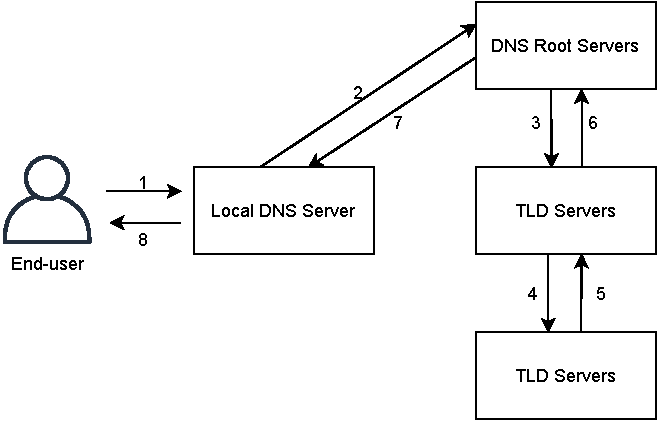
\includegraphics[width=\textwidth,trim={0 0 0 -0.5cm}]{figs/dns_routing.pdf}
        \centering
        \caption{DNS}
    \end{subfigure}
    \centering
    \begin{subfigure}[b]{0.45\textwidth}
        \centering
        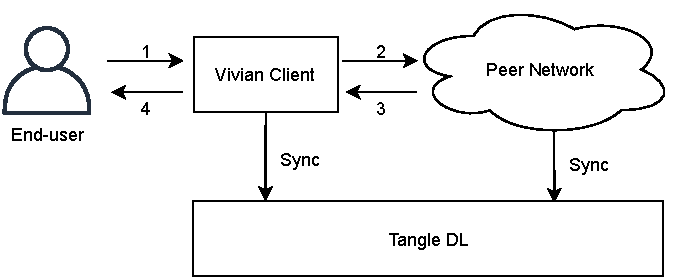
\includegraphics[width=\textwidth,trim={0 0 0 -0.5cm}]{figs/vivian_routing.pdf}
        \centering
        \caption{Vivian}
    \end{subfigure}
    \caption{Comparison of DNS and Vivian queries}
    \label{fig:query_compare}
\end{figure}

Through peer network routing layer, users can query the value of a name without relying on the trust of third parties.

\subsection{Storage System}
There is no restriction on what type of data a name should map to. The storage layer provides an alternative way for binding large files to the names.
Due to the data size limitation of Tangle transaction and complexity for checking the message content of the transaction, actual data are stored on the storage layer instead of Tangle DL.
Users can choose to use InterPlanetary File System (IPFS) \cite{benet2014ipfs}, a P2P decentralized file system, to save their files or traditional storage backends such as Amazon S3, Azure Blob, Google Cloud, etc.
The design goals are to let the users own the access right of their data, users do not need to trust the storage layer and can verify the data integrity, and the other third parties like the storage providers cannot tamper with the data.
Possible implementations will be discussed in Section~\ref{sec:implementation}.

\begin{figure*}[h]
    \centering
    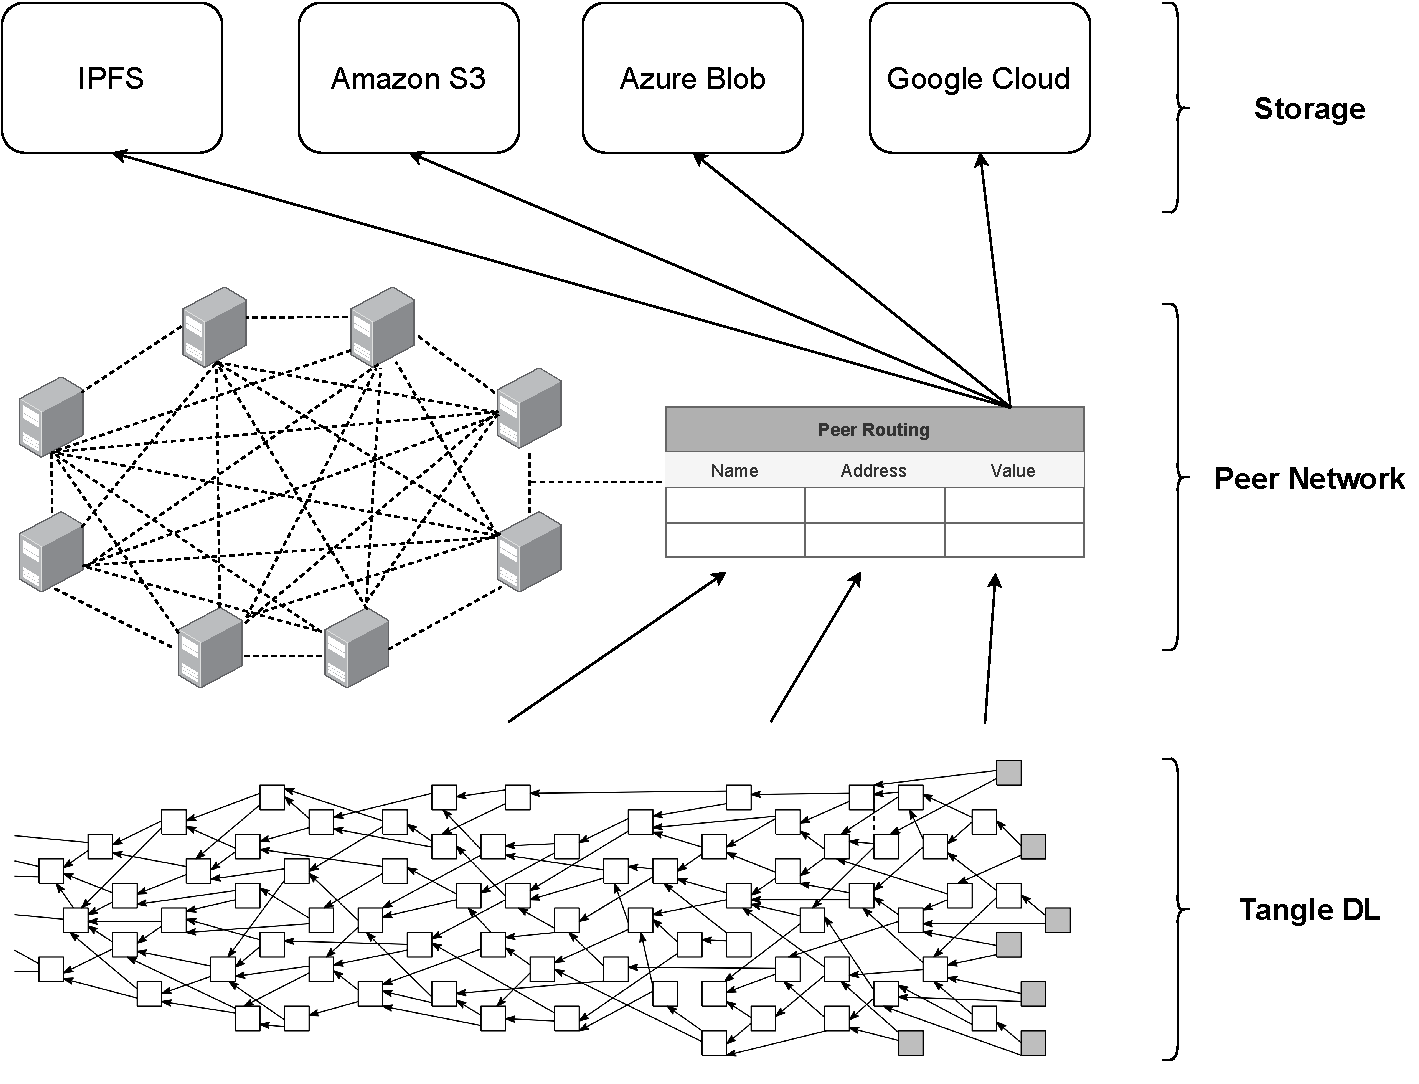
\includegraphics[width=0.8\textwidth,trim={0 0 0 0},clip]{figs/vivian_architecture.pdf}
    \caption{Vivian Architecture}
    \label{fig:vivian_architecture}
\end{figure*}